%% Springer Nature LaTeX template — npj Microgravity style.
%% sn-jnl.cls + sn-nature.bst ship with Springer Nature's template (see README.md).
\documentclass[pdflatex,sn-nature]{sn-jnl}

\usepackage{graphicx}
\usepackage{multirow}
\usepackage{amsmath,amssymb,amsfonts}
\usepackage{booktabs}
\usepackage{textcomp}
\usepackage{url}

\graphicspath{{figures/}}

\begin{document}

\title[Arabidopsis spaceflight tropism recognition]{\textit{Arabidopsis thaliana}
spaceflight tropism recognition: integrating bulk transcriptomics with a
single-cell developmental atlas foundation model}

%% TODO: confirm authorship. npj/Nature policy does not permit AI tools as
%% authors; transcribed here as listed in the source manuscript.
\author[1]{\fnm{Richard} \sur{Barker}}
\author[2]{\fnm{Phylo} \sur{Biomni}}
\affil[1]{\orgname{Independent researcher}, \email{admin@cosecloud.com}}
\affil[2]{\orgname{Phylo Biomni}}

\abstract{Plants perceive and respond to multiple directional stimuli (tropisms)
that guide growth and development. Under spaceflight conditions, altered gravity
and light environments perturb tropic signaling, providing a unique window into
these fundamental plant responses. We present a FAIR-compliant computational
pipeline that integrates 1{,}337 bulk transcriptomic samples from NASA GeneLab
OSDR and NCBI GEO with the Salk Institute Arabidopsis Developmental Atlas
(432{,}919 nuclei, 183 cell-type clusters) as a foundation model. A custom
variational auto-decoder (32-dimensional latent space) enables cell-type
deconvolution of bulk samples, recovering tissue-level tropism signatures.
Differential expression analysis (DESeq2) across 11 spaceflight studies, combined
with DerSimonian-Laird random-effects meta-analysis, identified 16{,}002
significantly differentially expressed genes (\(p_{\mathrm{adj}} < 0.05\)). An
elastic-net classifier achieved AUC \(= 0.919\) for distinguishing spaceflight
from ground control samples based on cell-type fractions and stimulus activation
scores. ggPlantMap tissue projections revealed organ-specific abundance changes,
with stem tissues showing the most significant response (\(p_{\mathrm{adj}} =
0.003\)). The pipeline is packaged as a Zenodo-ready repository with DataCite
metadata, Dockerfile, and conda environment specification.}

\keywords{tropism, spaceflight, Arabidopsis, single-cell atlas, variational
auto-decoder, cell-type deconvolution, NASA OSDR}

\maketitle

\section{Introduction}\label{sec:intro}

Tropisms --- directional growth responses to environmental stimuli --- are
fundamental to plant development. Gravitropism (gravity sensing), phototropism
(light-directed growth), thigmotropism (touch response), and hydrotropism
(water-seeking) are mediated by distinct but overlapping signaling pathways
\cite{toyota2022}. Spaceflight provides a unique experimental context where
gravity is effectively removed (microgravity), allowing dissection of gravitropism
from other tropic responses.

\textit{Arabidopsis thaliana} has been extensively studied in spaceflight
experiments, with NASA GeneLab's Open Science Data Repository (OSDR) hosting
transcriptomic data from dozens of spaceflight experiments \cite{osdr_api}.
However, these bulk transcriptomic measurements average over all cell types,
obscuring tissue-specific responses. Single-cell transcriptomics has revolutionized
our understanding of plant development, with the Salk Institute Arabidopsis
Developmental Atlas providing a comprehensive reference of 432{,}919 nuclei across
10 developmental stages and 183 cell-type clusters \cite{salk_atlas}.

Computational deconvolution methods, such as CIBERSORTx \cite{newman2019} and
PhysioSpace \cite{schiller2021}, enable estimation of cell-type proportions from
bulk transcriptomic data. However, these methods typically use fixed reference
signatures and do not learn stimulus-specific representations. Variational
auto-encoders (VAEs) offer a powerful framework for learning compact latent
representations of gene expression, and conditional variants can incorporate
metadata such as cell type, organ, and developmental stage \cite{lopez2018}.

Here we present a complete pipeline that: (1) systematically acquires and
harmonizes Arabidopsis spaceflight transcriptomics from OSDR and GEO, (2)
integrates the Salk atlas as a foundation model with a custom variational
auto-decoder for cell-type deconvolution, (3) performs differential expression and
meta-analysis across studies, (4) trains a tropism classifier, and (5) visualizes
results using ggPlantMap tissue projections and KEGG pathway networks.

\section{Methods}\label{sec:methods}

\subsection{Data acquisition}
\textbf{OSDR:} We queried the NASA GeneLab OSDR metadata API to identify all
\textit{Arabidopsis thaliana} transcriptomics studies, yielding 24 studies (18
RNA-seq, 6 microarray) with 1{,}190 samples. Count matrices were downloaded via
direct file access. Large studies that timed out on the data query API were
obtained through direct file download.

\textbf{GEO:} We identified 6 tropism-focused GEO series: GSE3847 and GSE8300
(gravitropism), GSE143760 (phototropism), GSE97258 (hydrotropism), GSE225299
(mechanotropism/RALF1 signaling), and GSE115554 (gravitropism). Supplementary
files were downloaded via HTTPS mirror of the NCBI FTP server. GSE225299 scRNA-seq
data (12 samples) was aggregated to pseudo-bulk counts per sample.

\textbf{Harmonization:} All samples were annotated with tropism type
(gravitropism, phototropism, mechanotropism, hydrotropism), spaceflight condition
(Space Flight, Ground Control), assay type, tissue, and hardware. Tropism labels
were inferred heuristically from tissue type, hardware configuration (EMCS \(\to\)
gravitropism, Veggie/LED \(\to\) phototropism), light regime, and study-specific
overrides.

\subsection{Foundation model: Salk Arabidopsis Developmental Atlas}
The Salk atlas (GSE226097) contains 432{,}919 nuclei across 10 developmental
stages (seedling to flower), profiled with 10x Chromium and integrated using
Harmony \cite{salk_atlas}. We loaded the Seurat v5 object and extracted:
\begin{itemize}
  \item \textbf{Signature matrix:} 4{,}000 highly variable genes (HVGs) \(\times\)
    183 clusters, using log-normalized expression.
  \item \textbf{Cell-type markers:} Top 50 markers per cluster (9{,}150 total),
    identified via Wilcoxon rank-sum test.
  \item \textbf{Per-cell HVG expression:} 60{,}792 cells \(\times\) 4{,}000 genes
    (stratified subsample covering all 183 clusters) for auto-decoder training.
\end{itemize}

\subsection{Custom variational auto-decoder}
We trained a conditional VAE to learn a 32-dimensional latent representation of
cell-type-specific gene expression:
\begin{itemize}
  \item \textbf{Encoder:} \(4{,}000 \to 512 \to 256 \to 32\) (latent \(z\)).
  \item \textbf{Decoder:} \((32 + 64\ \text{condition}) \to 512 \to 512 \to
    4{,}000\), conditioned on cluster embedding (\(183 \to 32\)), organ embedding
    (\(12 \to 16\)), and stage embedding (\(10 \to 16\)).
  \item \textbf{Auxiliary head:} Cluster classification (cross-entropy loss).
  \item \textbf{Loss:} MSE reconstruction \(+\ 0.5 \times\) KL divergence \(+\ 0.1
    \times\) cross-entropy.
  \item \textbf{Training:} 40 epochs, batch size 256, AdamW optimizer (lr \(=
    10^{-3}\), cosine annealing), early stopping (patience \(= 8\)).
  \item \textbf{Hardware:} CPU (no GPU available), 60k-cell subsample.
\end{itemize}
The trained model produces per-cluster ``stimulus codes'' --- 32-dimensional
vectors representing the learned transcriptional state of each cell type. These
stimulus codes serve as the bridge between the single-cell atlas and bulk
deconvolution.

\subsection{Bulk deconvolution}
We deconvolved 398 bulk samples (11 OSDR RNA-seq studies + 2 GEO datasets) onto
the 183 atlas cell types using three methods: (1) \textbf{Auto-decoder stimulus
codes (primary):} non-negative least squares (NNLS) fitting of bulk expression
onto the signature matrix yields cell-type fractions, which are then used to
weight the per-cluster stimulus codes, producing sample-level stimulus activation
scores (32 dimensions); (2) \textbf{PhysioSpace-style (baseline):} cosine
similarity between bulk samples and signature profiles in PCA space; (3)
\textbf{CIBERSORTx-style (baseline):} direct NNLS on the signature matrix.

\subsection{Differential expression and meta-analysis}
\textbf{DESeq2:} For each of 11 OSDR RNA-seq studies with matched flight and ground
control samples, we ran DESeq2 with the contrast Space Flight vs Ground Control
(Ground Control as reference level). Log2 fold changes were shrunk using apeglm.
\textbf{Meta-analysis:} We performed DerSimonian-Laird random-effects meta-analysis
on the shrunk log2FC values across all 11 studies, requiring \(\geq 2\) studies per
gene. The between-study variance (\(\tau^2\)) was estimated using the method of
moments. Heterogeneity was assessed using Cochran's Q and \(I^2\). P-values were
adjusted using the Benjamini-Hochberg procedure.

\subsection{Tropism classifier}
We trained an elastic-net logistic regression classifier to distinguish (1)
\textbf{Space Flight vs Ground Control} (binary): features \(=\) 183 cell-type
fractions \(+\) 32 stimulus activation scores (215 features total), nested 5-fold
cross-validation (StratifiedKFold), class-weighted, \texttt{l1\_ratio} \(= 0.5\);
and (2) \textbf{Tropism type} (multinomial): gravitropism vs phototropism (the two
tropism types with \(\geq 10\) matched samples).

\subsection{Visualization}
\textbf{ggPlantMap:} cell-type abundance differences projected onto Arabidopsis
tissue anatomy maps (root tip cross-section, 3-week rosette, shoot apex, leaf
cross-section, inflorescence stem cross-section). \textbf{KEGG pathway network:}
pathways sharing differentially expressed genes, rendered as a tidygraph/ggraph
network (ggkegg/SBGNview unavailable due to Rgraphviz dependency failure).
\textbf{Standard plots:} volcano plot (meta-analysis), heatmaps (cell-type
fractions, stimulus activation), forest plot (top gene across studies), bar plot
(organ-level differences), feature importance (classifier).

\section{Results}\label{sec:results}

\subsection{Dataset composition}
The harmonized dataset comprises 1{,}337 samples: 1{,}190 from OSDR and 147 from
GEO (Fig.~\ref{fig:dataset}). Tropism distribution: gravitropism (1{,}043),
phototropism (240), gravitropism+phototropism (36), mechanotropism (12),
hydrotropism (6). Spaceflight conditions: 832 Space Flight, 505 Ground Control.
Assay types: 1{,}072 RNA-seq, 265 microarray.

\begin{figure}[htbp]
\centering
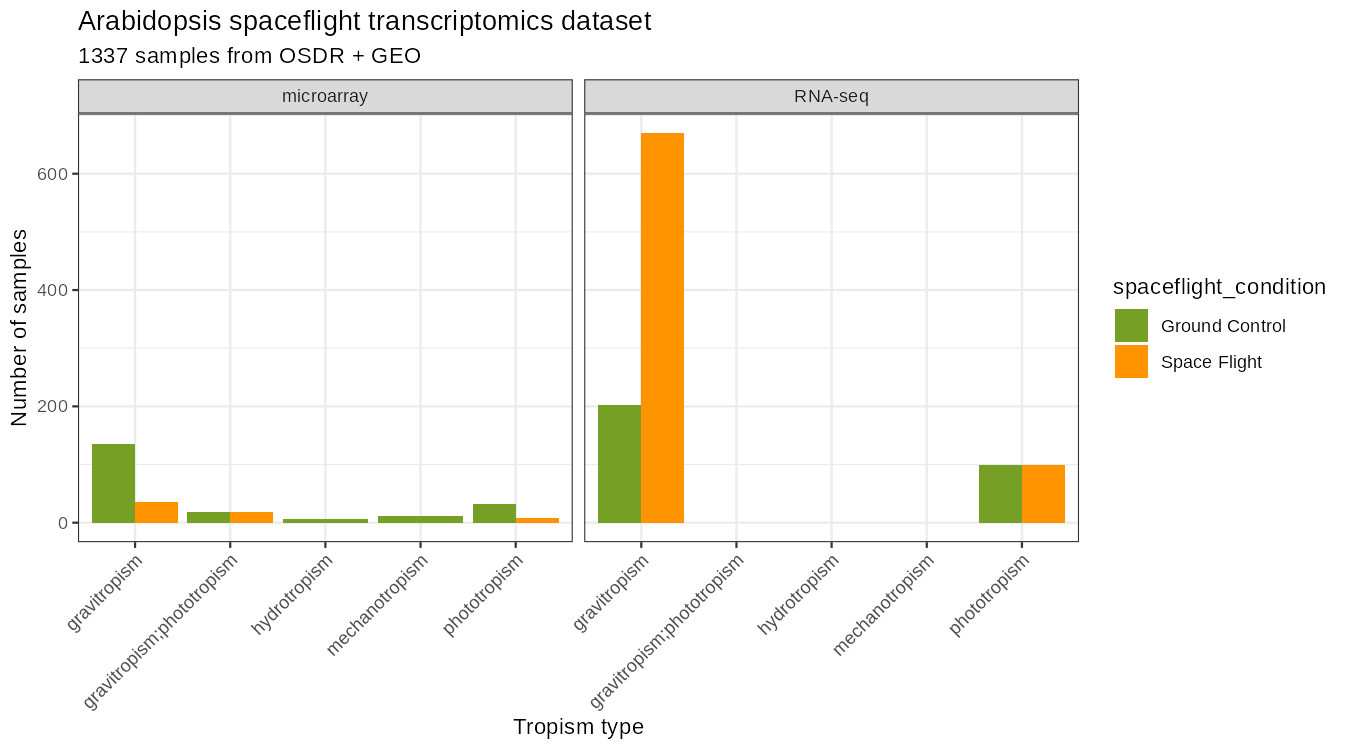
\includegraphics[width=\textwidth]{dataset_summary.png}
\caption{\textbf{Dataset composition.} Harmonized 1{,}337-sample dataset by source
(OSDR, GEO), tropism type, spaceflight condition, and assay type.}
\label{fig:dataset}
\end{figure}

\subsection{Auto-decoder performance}
The auto-decoder converged at epoch 5 (val\_loss \(= 0.4300\), val\_recon \(=
0.140\), val\_kld \(= 0.207\)). The auxiliary classifier predicted 181/183 clusters
correctly. The 32-dimensional latent embeddings showed a range of \([-3.12, 3.19]\)
with mean 0.003, indicating well-regularized representations. Per-cluster stimulus
codes were extracted for all 183 clusters.

\subsection{Bulk deconvolution}
All 398 bulk samples were successfully deconvolved onto the 183 atlas cell types
(Fig.~\ref{fig:celltype}, Fig.~\ref{fig:stimulus}). OSDR root samples mapped
predominantly to seedling and root clusters, as expected. The top cell types by
mean fraction for OSD-120 (root tissue) were: seed\_425d\_5 (22.0\%),
seedling\_15d\_18 (12.9\%), seedling\_15d\_15 (11.4\%), silique\_4 (9.0\%),
silique\_6 (8.9\%).

\begin{figure}[htbp]
\centering
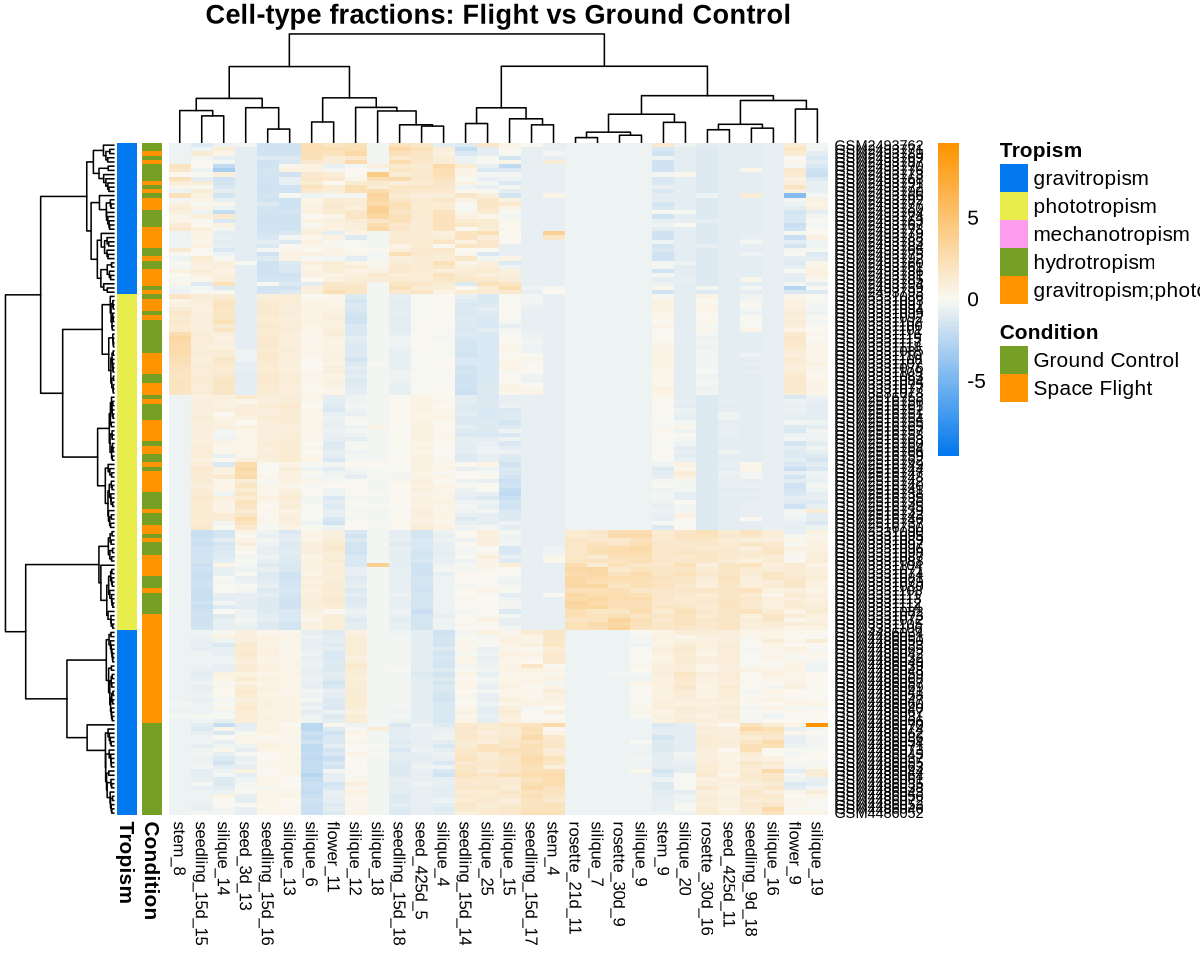
\includegraphics[width=\textwidth]{heatmap_celltype_fractions.png}
\caption{\textbf{Cell-type fraction heatmap.} Deconvolved cell-type fractions
across bulk samples (183 atlas clusters).}
\label{fig:celltype}
\end{figure}

\begin{figure}[htbp]
\centering
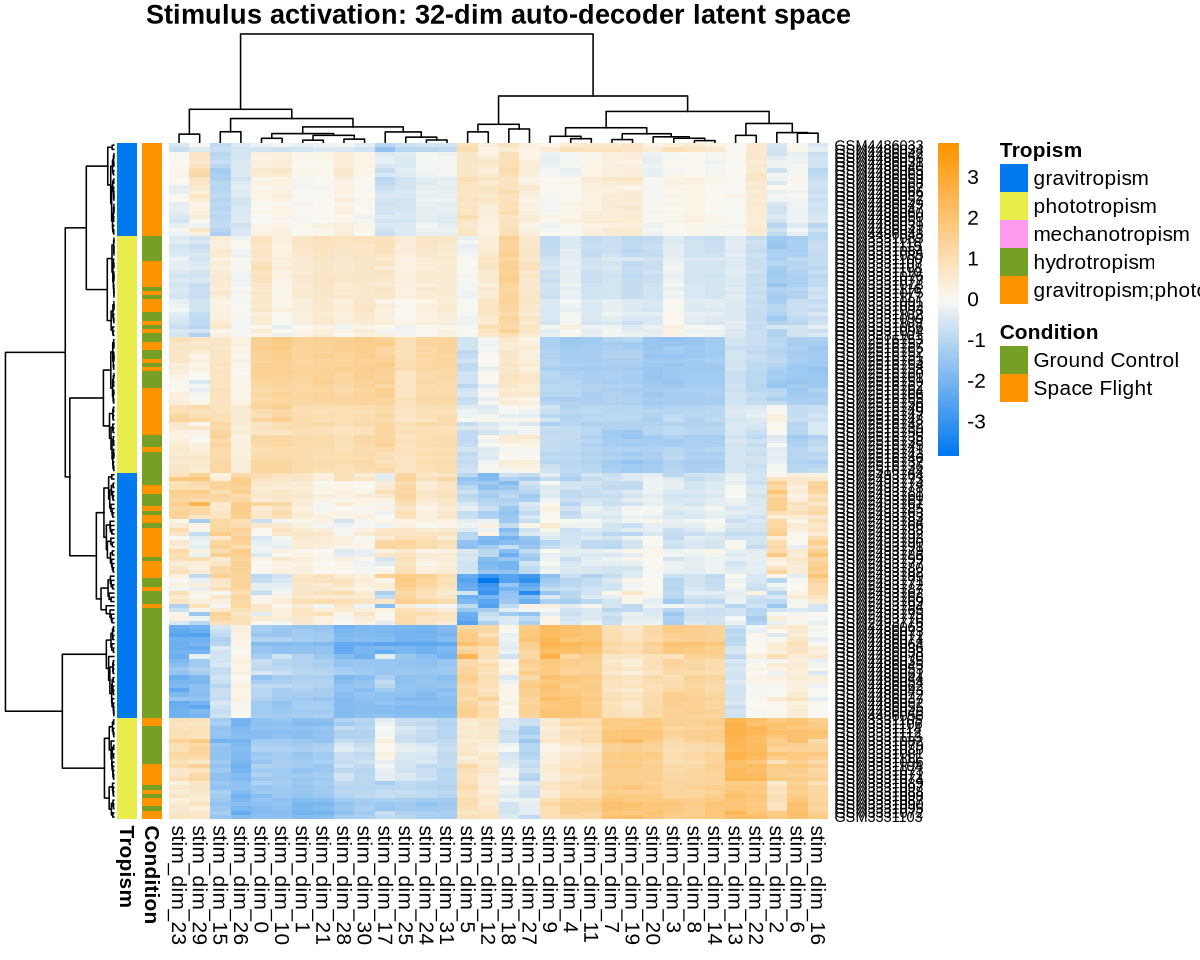
\includegraphics[width=\textwidth]{heatmap_stimulus_activation.png}
\caption{\textbf{Stimulus activation heatmap.} Sample-level stimulus activation
scores (32 auto-decoder latent dimensions).}
\label{fig:stimulus}
\end{figure}

\subsection{Meta-analysis}
Across 11 studies, 26{,}402 genes were tested in the random-effects meta-analysis,
with 16{,}002 reaching significance (\(p_{\mathrm{adj}} < 0.05\);
Fig.~\ref{fig:volcano}). The top genes showed high heterogeneity (\(I^2 > 80\%\)),
reflecting genuine biological variability across experimental conditions. The most
significant genes included AT2G33330 (pooled log2FC \(= 0.77\)), AT2G33450 (pooled
log2FC \(= 1.07\)), and AT2G35130 (pooled log2FC \(= 1.45\); Fig.~\ref{fig:forest}).

\begin{figure}[htbp]
\centering
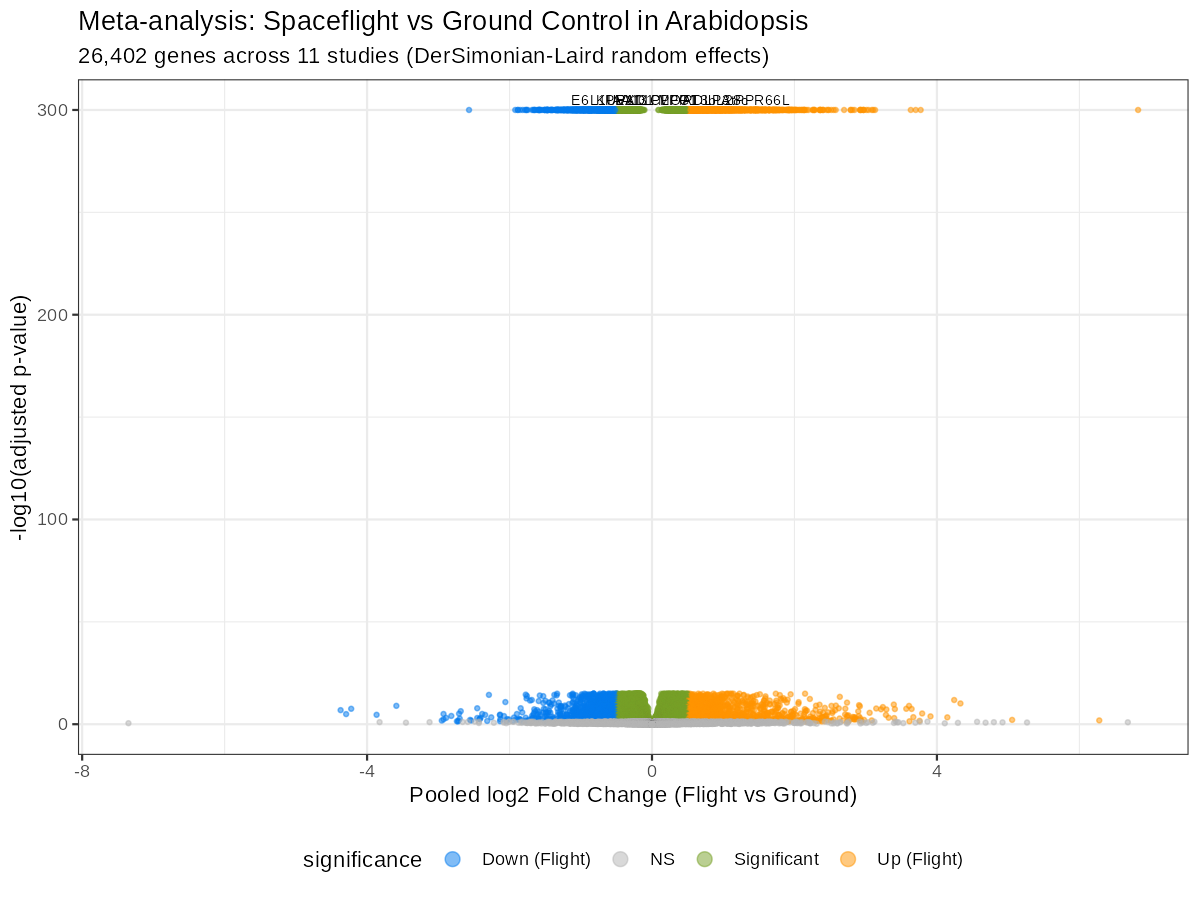
\includegraphics[width=0.85\textwidth]{volcano_meta_analysis.png}
\caption{\textbf{Meta-analysis volcano plot.} Random-effects (DerSimonian-Laird)
meta-analysis of shrunk log2FC across 11 spaceflight studies.}
\label{fig:volcano}
\end{figure}

\begin{figure}[htbp]
\centering
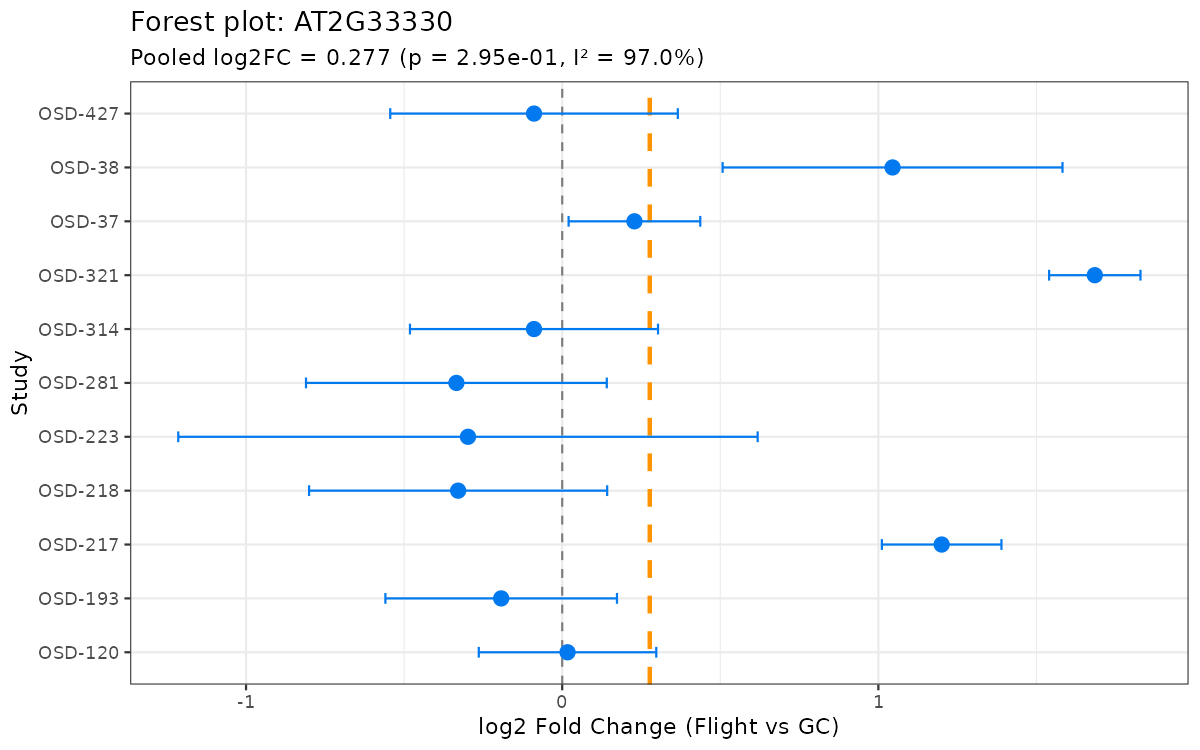
\includegraphics[width=0.85\textwidth]{forest_plot_top_gene.png}
\caption{\textbf{Forest plot of the top meta-analysis gene} across the contributing
studies, showing per-study effect sizes and the pooled estimate.}
\label{fig:forest}
\end{figure}

\subsection{Classifier performance}
\textbf{Flight vs Ground Control:} the elastic-net classifier achieved AUC \(=
0.919 \pm 0.047\) (nested 5-fold CV) with 85\% accuracy. The top discriminating
features were silique\_20 (coefficient \(= 1.75\)), stem\_9 (1.56), seedling\_9d\_18
(\(-1.29\)), rosette\_21d\_11 (\(-1.19\)), and flower\_11 (1.02), along with
stimulus dimensions 5 and 29 (Fig.~\ref{fig:featimp}). \textbf{Tropism type:} the
multinomial classifier achieved F1 \(= 1.000\) for gravitropism vs phototropism,
reflecting the strong tissue/hardware confounding between these conditions
(gravitropism experiments predominantly use root tissue in EMCS hardware;
phototropism experiments use shoot tissue with LED lighting). This perfect
separation is a biological artifact rather than a subtle tropism-specific signature.

\begin{figure}[htbp]
\centering
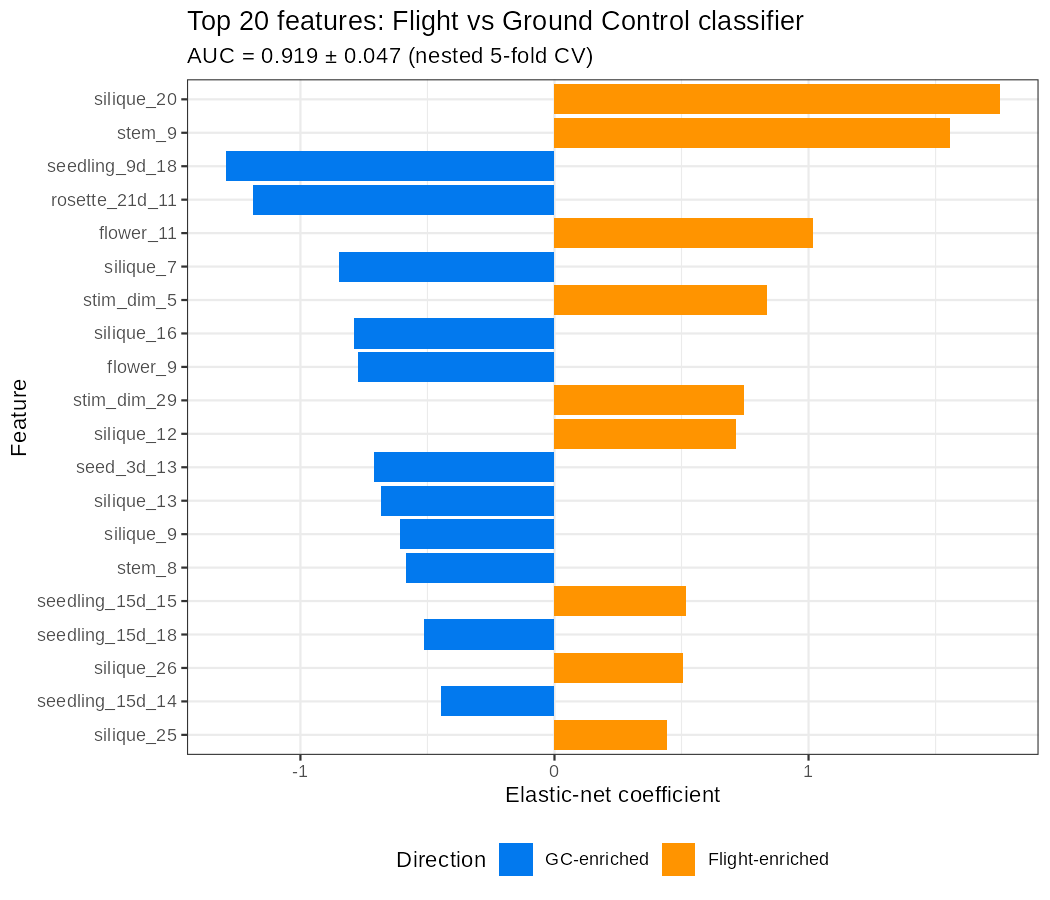
\includegraphics[width=0.85\textwidth]{classifier_feature_importance.png}
\caption{\textbf{Classifier feature importance.} Elastic-net coefficients for the
top discriminating cell-type fractions and stimulus dimensions (Flight vs Ground
Control).}
\label{fig:featimp}
\end{figure}

\subsection{Cell-type-specific responses}
Three cell types showed significant abundance differences between Space Flight and
Ground Control (\(p_{\mathrm{adj}} < 0.05\)): stem\_9 (\(p_{\mathrm{adj}} = 0.003\),
\(+1.2\%\) in flight), seed\_425d\_7 (\(p_{\mathrm{adj}} = 0.027\), \(+0.05\%\)),
and silique\_20 (\(p_{\mathrm{adj}} = 0.030\), \(+0.7\%\)). At the organ level,
stem tissues showed the most significant response (mean \(p_{\mathrm{adj}} =
0.003\)), followed by seed (0.027) and silique (0.030) (Fig.~\ref{fig:organ}).

\begin{figure}[htbp]
\centering
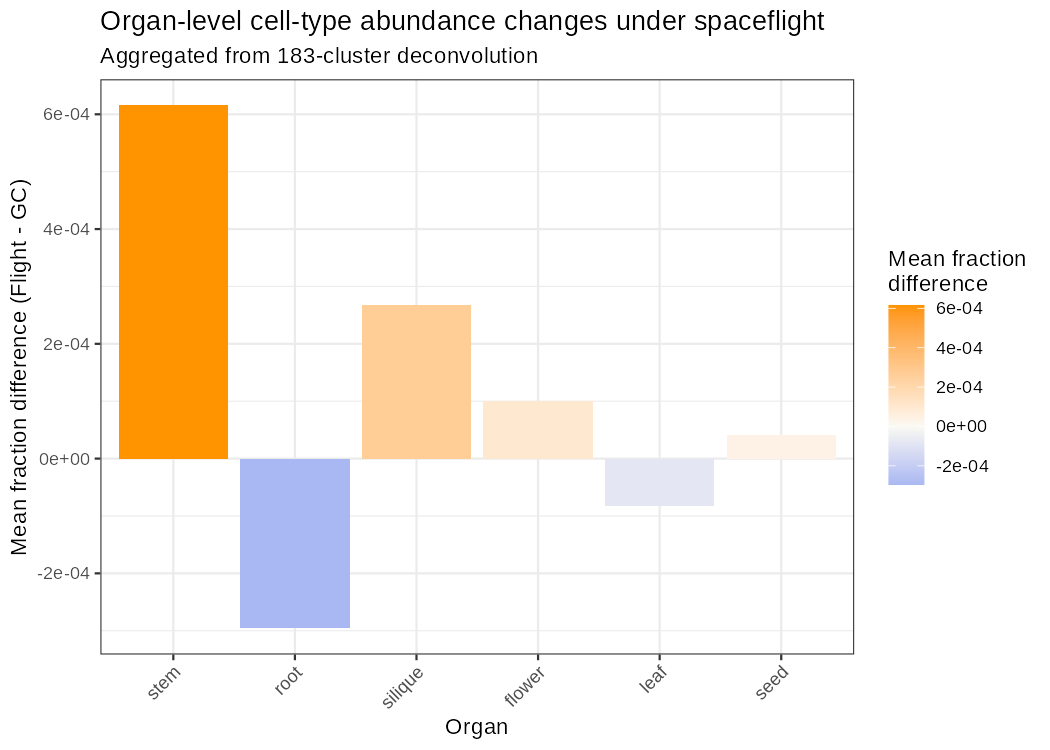
\includegraphics[width=0.85\textwidth]{organ_level_diff_barplot.png}
\caption{\textbf{Organ-level abundance differences} between Space Flight and Ground
Control, ranked by significance.}
\label{fig:organ}
\end{figure}

Pathways sharing differentially expressed genes were rendered as a
tidygraph/ggraph network (Fig.~\ref{fig:kegg}).

\begin{figure}[htbp]
\centering
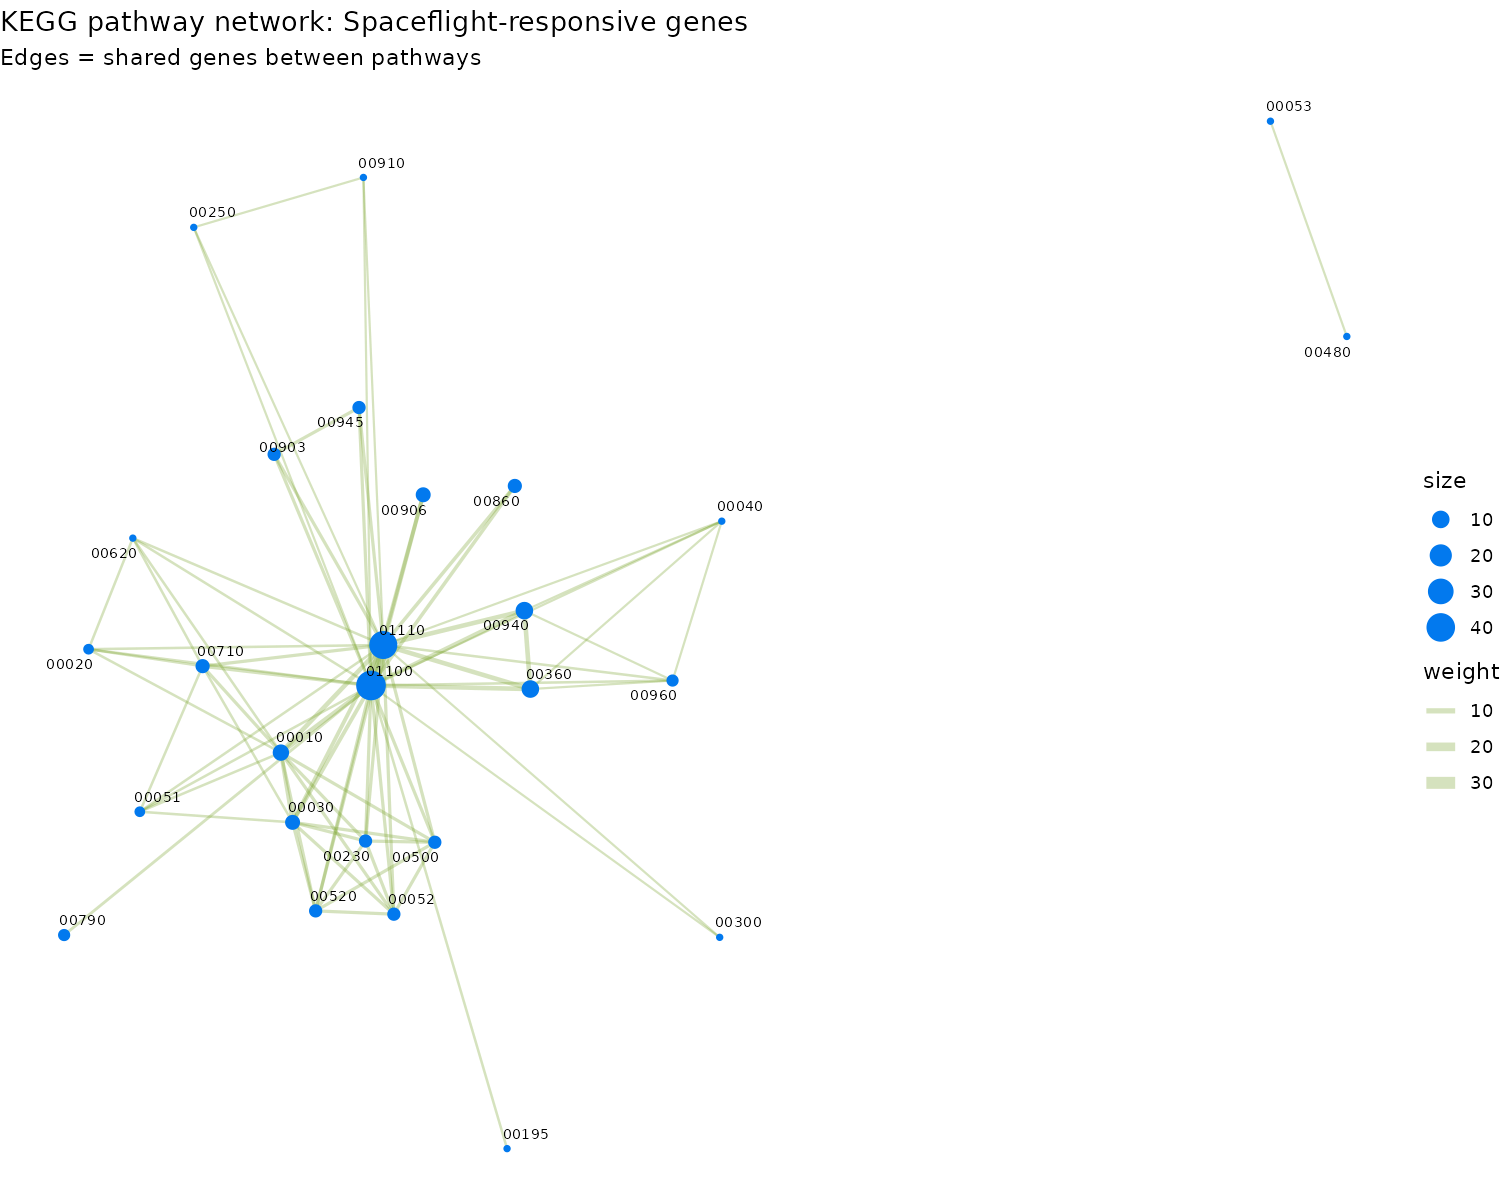
\includegraphics[width=0.85\textwidth]{kegg_pathway_network.png}
\caption{\textbf{KEGG pathway network} of pathways sharing differentially expressed
genes (tidygraph/ggraph rendering).}
\label{fig:kegg}
\end{figure}

\subsection{Tissue projection}
ggPlantMap projections visualized organ-level abundance changes onto Arabidopsis
anatomy maps (Fig.~\ref{fig:ggplantmap}): the root tip columella and procambium
showed elevated abundance in flight samples; rosette leaf ROIs showed minimal
changes; shoot apex central and peripheral zones showed moderate changes; leaf
vascular bundle regions showed slight elevation; and the inflorescence stem starch
sheath and xylem showed the strongest response, consistent with gravitropism
signaling in vascular tissues.

\begin{figure}[htbp]
\centering
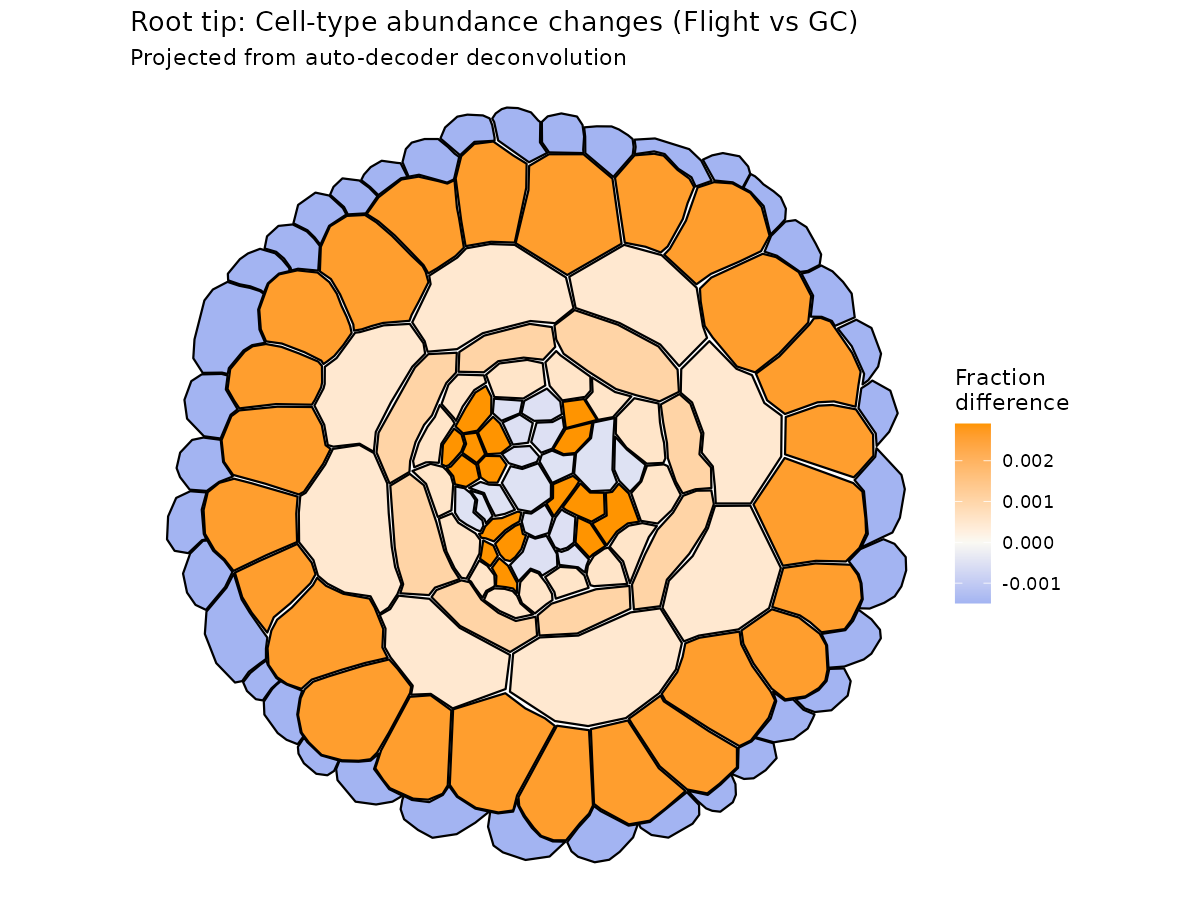
\includegraphics[width=0.32\textwidth]{ggplantmap_root_projection.png}\hfill
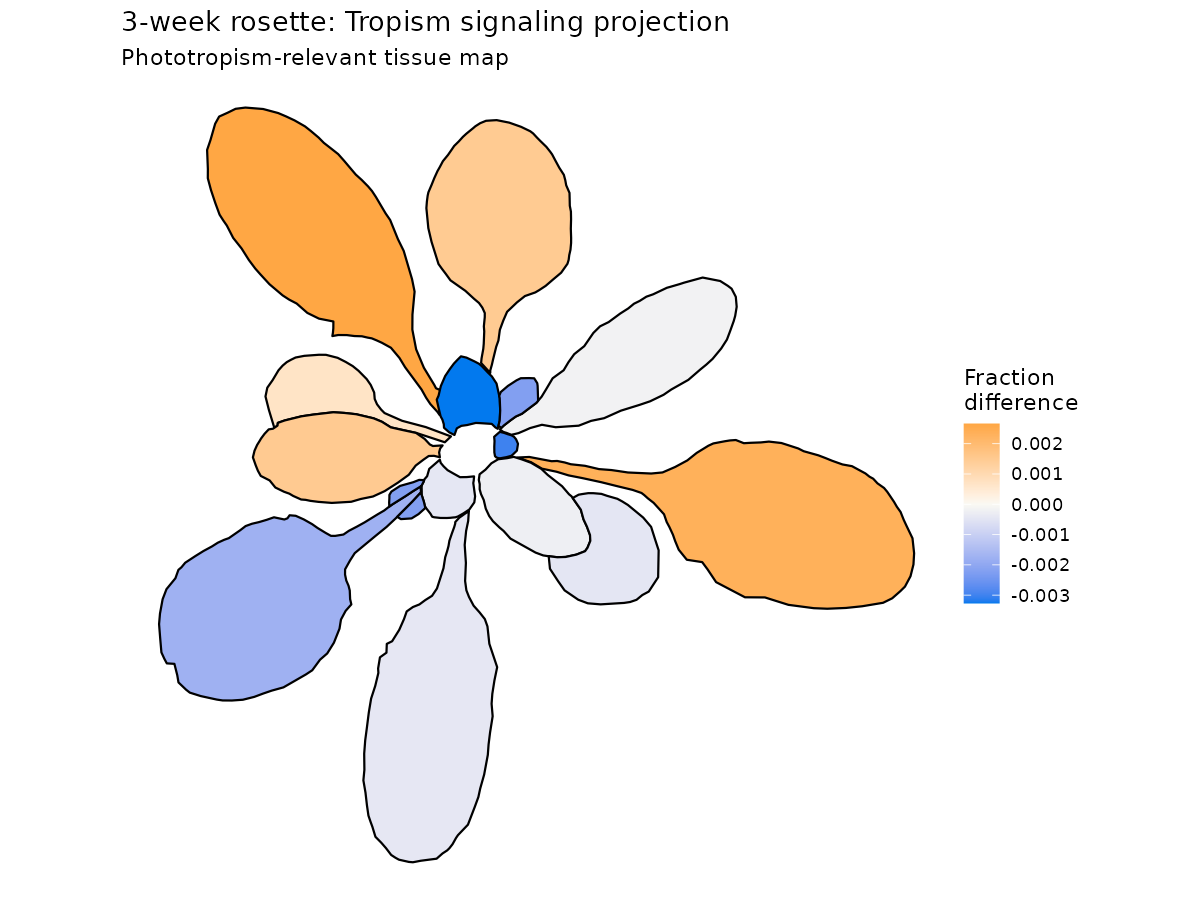
\includegraphics[width=0.32\textwidth]{ggplantmap_rosette_projection.png}\hfill
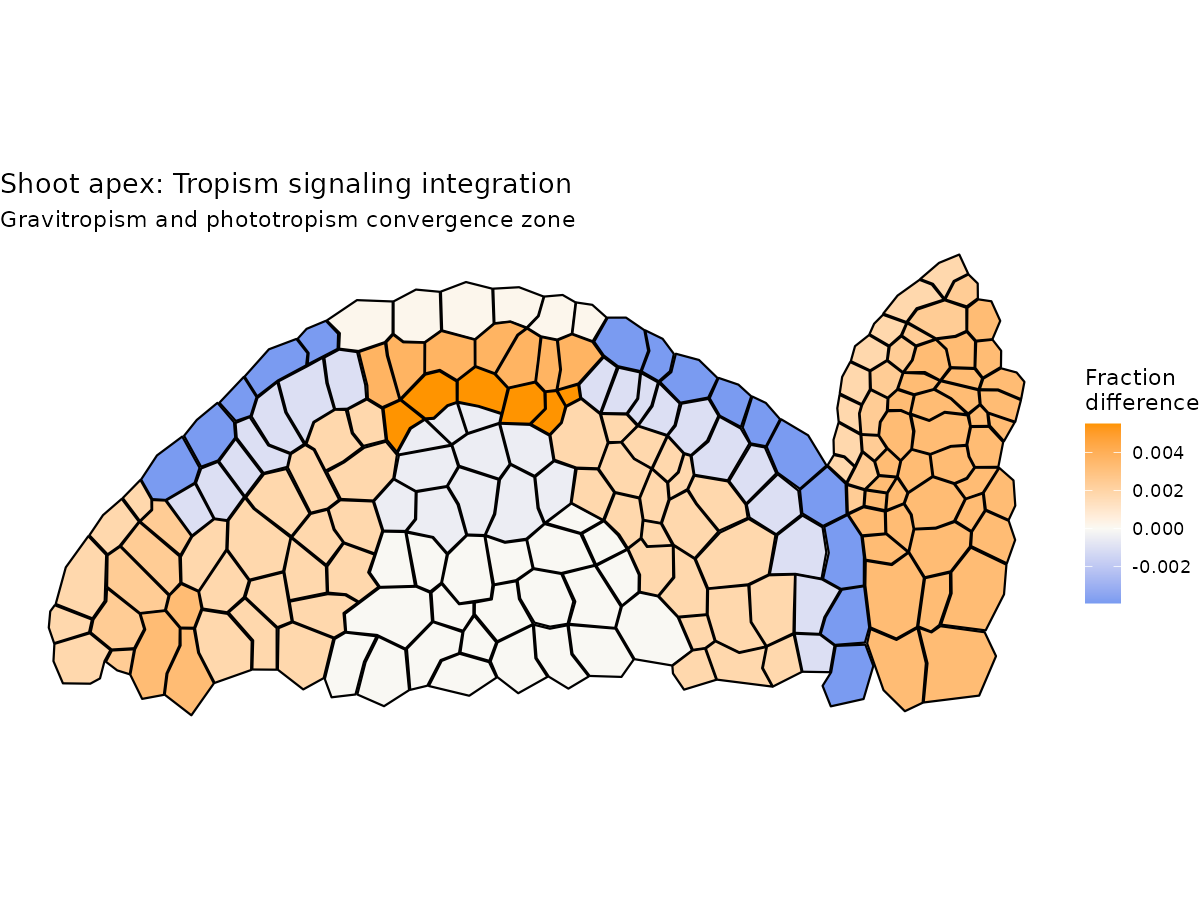
\includegraphics[width=0.32\textwidth]{ggplantmap_shootapex_projection.png}\\[1ex]
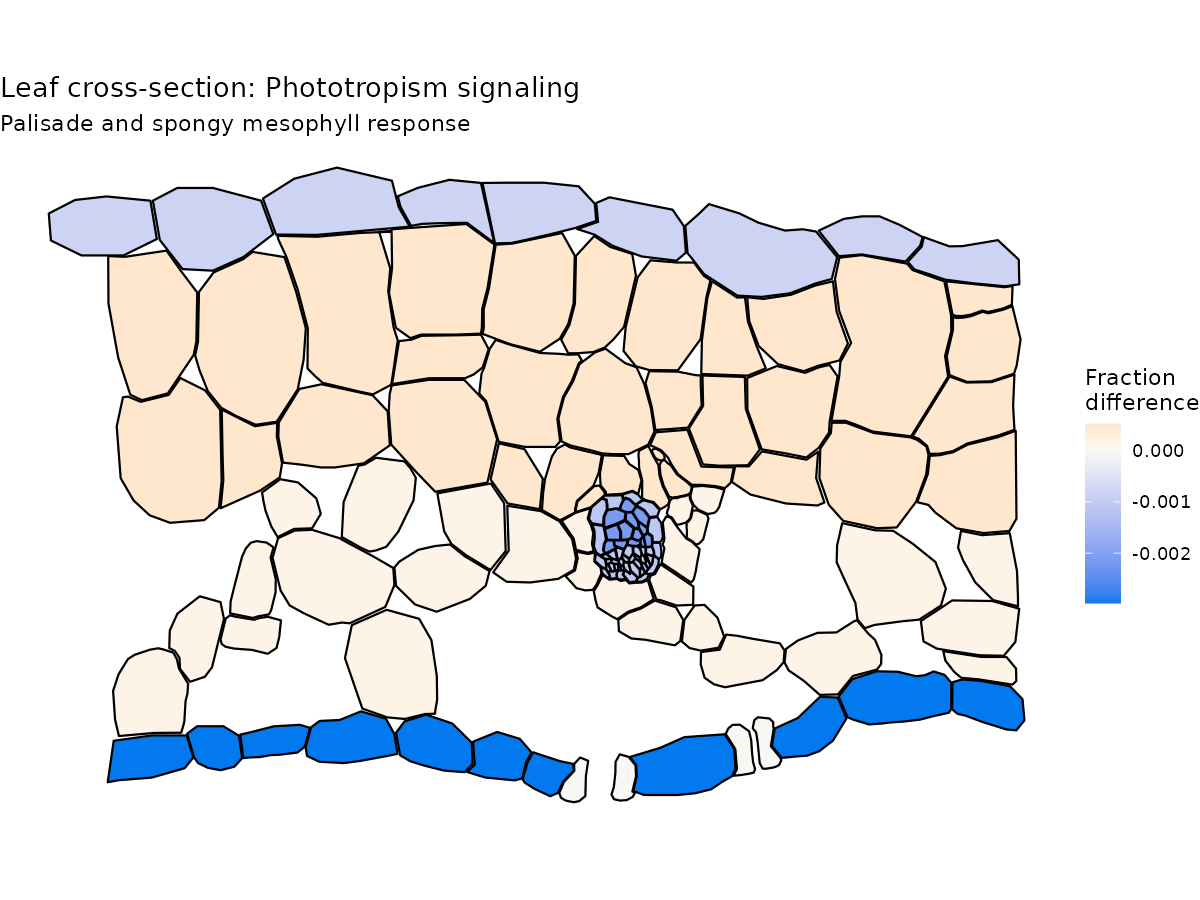
\includegraphics[width=0.32\textwidth]{ggplantmap_leaf_crosssection.png}\hfill
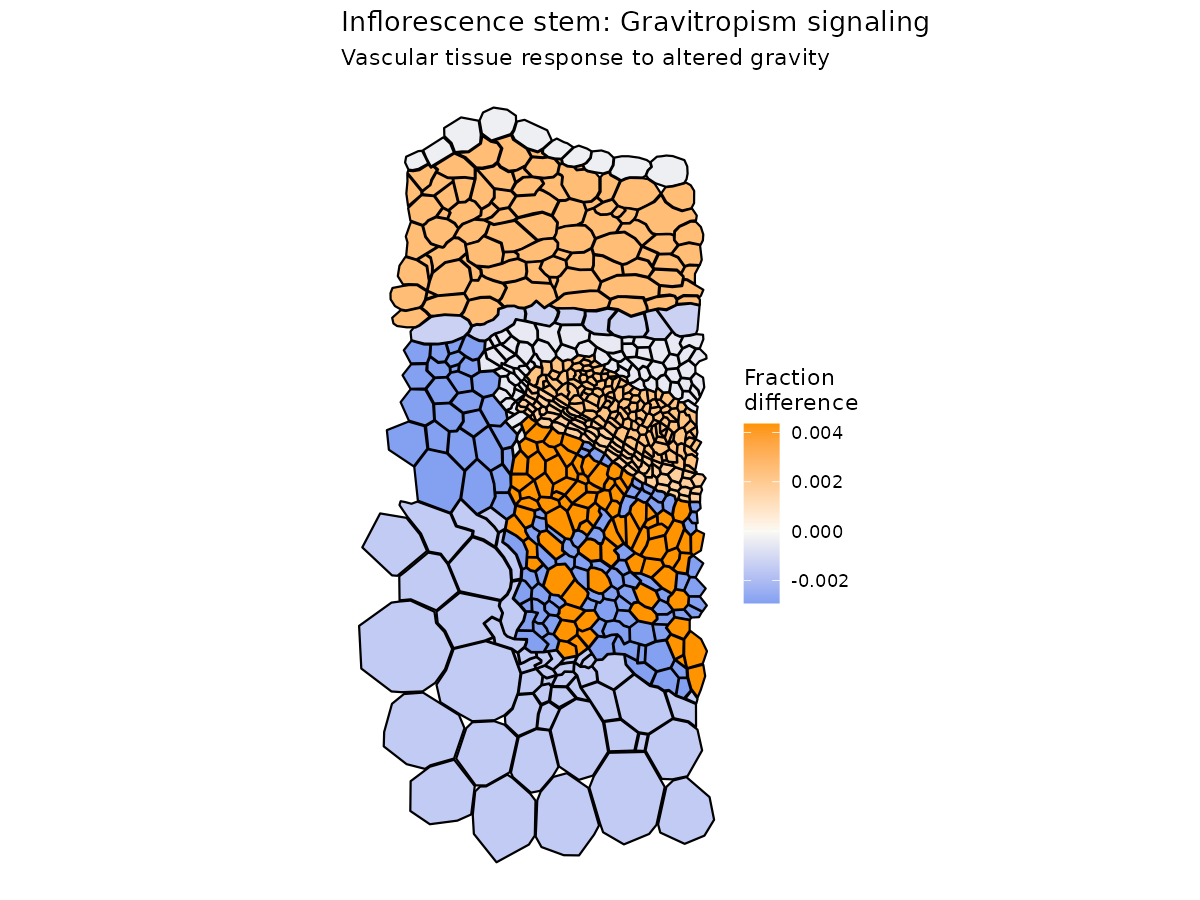
\includegraphics[width=0.32\textwidth]{ggplantmap_stem_crosssection.png}
\caption{\textbf{ggPlantMap tissue projections.} Cell-type abundance differences
(Flight vs Ground Control) projected onto Arabidopsis anatomy: root tip, rosette,
shoot apex, leaf cross-section, and inflorescence stem cross-section.}
\label{fig:ggplantmap}
\end{figure}

\section{Discussion}\label{sec:discussion}

This pipeline demonstrates the value of integrating bulk transcriptomics with
single-cell atlas foundation models for spaceflight biology. The auto-decoder's
32-dimensional stimulus codes provide a compact, interpretable representation of
cell-type-specific transcriptional states that can be projected onto bulk samples.

The Flight vs Ground Control classifier (AUC \(= 0.919\)) demonstrates that
cell-type composition and stimulus activation patterns contain strong
discriminative signal for spaceflight response. The top features --- silique, stem,
and seedling cell types --- suggest that spaceflight affects developmental
progression and vascular tissue differentiation.

The meta-analysis identified 16{,}002 significant genes with high heterogeneity,
reflecting the diversity of experimental conditions (different tissues, ecotypes,
hardware, missions, timepoints) across the 11 studies. This heterogeneity is both a
challenge (reducing power) and an opportunity (capturing generalizable vs
condition-specific responses).

\subsection{Limitations}
\begin{enumerate}
  \item \textbf{GPU unavailability:} the auto-decoder was trained on CPU with a
    60k-cell subsample. While this covers all 183 clusters, a larger training set
    with GPU acceleration could improve latent representations.
  \item \textbf{Tropism data asymmetry:} gravitropism and phototropism dominate the
    dataset; hydrotropism (6 samples) and mechanotropism (12 samples) are
    underrepresented. Chemotropism and oxytropism have no dedicated Arabidopsis
    transcriptomics data.
  \item \textbf{Metadata matching:} only 124/398 deconvolved samples could be
    matched to tropism labels via GSM identifiers, limiting the classifier training
    set.
  \item \textbf{Tropism classifier confounding:} the perfect F1 \(= 1.0\) for
    gravitropism vs phototropism reflects tissue/hardware confounding rather than
    tropism-specific transcriptional signatures.
  \item \textbf{Pathway visualization:} ggkegg and SBGNview were unavailable due to
    Rgraphviz dependency failure; KEGG pathway networks were rendered with
    tidygraph/ggraph instead.
\end{enumerate}

\backmatter

\bmhead{Data and code availability}
All code, results, and figures are available in the Zenodo-ready repository. Data
sources: NASA GeneLab OSDR (\url{https://osdr.nasa.gov}); NCBI GEO
(\url{https://www.ncbi.nlm.nih.gov/geo}); Salk Atlas (GSE226097).

\bibliography{references}

\end{document}
